\chapter{Diseño para Máxima Excursión Simétrica}
En la Figura \ref{fig:amplificador} se muestra el circuito utilizado en el presente trabajo práctico. El mismo consiste
en un amplificador basado en un transistor BJT en configuración emisor común con 
polarización mediante divisor resistivo. Esta topología se caracteriza por permitir un punto de operación
estable frente a variaciones del $\beta$. 
El circuito incluye las resistencias $R_1$, $R_2$, $R_E$, $R_C$ y $R_L$, junto a capacitores de desacople y una fuente de 
alimentación $V_{CC}$. Algunos de estos valores fueron fijados por las consignas del trabajo.

\begin{figure}[!ht]
    \centering
    \begin{tikzpicture}
      \node[npn](N1) at (9.25, 5.75){} node[anchor=west] at (N1.text){$Q1$};
      \draw (7, 5) to[american resistor, l={$R_1$}] (7, 2.75);
      \draw (7, 5.75) to[capacitor, l={$C_1$}] (3, 5.75);
      \draw (7, 5.75) -- (8.41, 5.75);
      \draw (9.25, 5) to[american resistor, l={$R_E$}] (9.25, 2.75);
      \draw (3, 5.75) to[sinusoidal voltage source, l={$v_i$}] (3, 2.5);
      \draw (7, 8.75) to[american resistor, l={$R_2$}, name=R1] (7, 6.5);
      \draw (9.25, 8.77) to[american resistor, l={$R_C$}] (9.25, 6.52);
      \draw (7, 5) -| (7, 6.5);
      \draw (11, 5) to[capacitor, l={$C_E$}] (11, 2.75);
      \draw (9.25, 5) -- (11, 5);
      \draw (7, 8.75) -| (7, 9) -| (9.25, 8.77);
      \draw (11, 2.75) |- (7, 2.5) -| (7, 2.75);
      \draw (9.25, 2.75) -| (9.25, 2.5);
      \draw (3, 2.5) -- (7, 2.5);
      \draw (10.25, 6.5) to[capacitor, l={$C_2$}] (13, 6.5);
      \draw (13.75, 5.5) to[american resistor, l={$R_L$}] (13.75, 3.25);
      \draw (13.75, 6.5) -| (13.75, 5.5);
      \draw (11, 2.5) -| (13.75, 3.25);
      \node[vcc](N2) at (9.25, 9.75){} node[anchor=south] at (N2.text){$V_{CC}$};
      \draw (9.25, 9) -| (9.25, 9.75);
      \node[ground] at (9.25, 2){};
      \draw (9.25, 2.5) -| (9.25, 2);
      \draw (10.25, 6.5) -- (9.25, 6.5);
      \draw (13, 6.5) -- (13.75, 6.5);
    \end{tikzpicture}
    \caption{amplificador emisor común.}
    \label{fig:amplificador}
\end{figure}

El objetivo de esta sección es establecer las condiciones de polarización en corriente continua de 
manera que el transistor opere en la región activa, garantizando linealidad en la 
amplificación de señales pequeñas. En particular, se busca ubicar el punto de operación $Q$ 
en la recta de carga de tal forma que la señal de salida pueda desplazarse con la mayor 
amplitud posible antes de alcanzar las regiones de saturación o corte.

Este criterio se conoce como polarización para máxima excursión simétrica (MES). Consiste 
en ajustar el punto de operación en el centro de las características de salida del transistor, 
de modo que la señal alterna pueda oscilar con igual margen hacia arriba y hacia abajo, 
evitando distorsiones. La Figura \ref{fig:gráfica-mes} ilustra este concepto, donde se observa el punto 
$Q_{MES}$, así como la comparación entre la recta de carga de continua y la de alterna.


\begin{figure}[!ht]
    \centering
    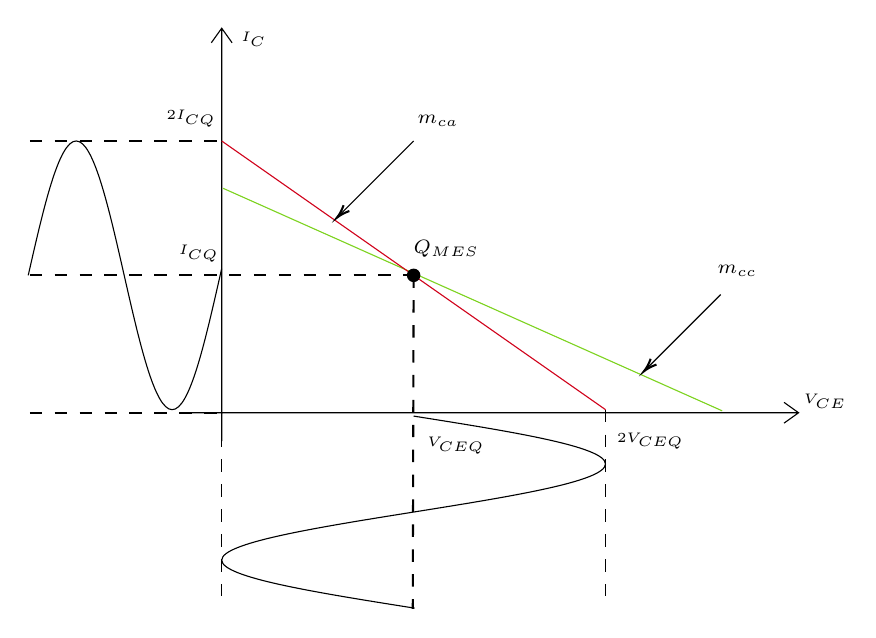
\begin{tikzpicture}[x=0.75pt,y=0.75pt,yscale=-1,xscale=1]
    %uncomment if require: \path (0,538); %set diagram left start at 0, and has height of 538
    
    %Shape: Axis 2D [id:dp5849296416796758] 
    \draw  (178.6,264.42) -- (472.39,264.42)(194.46,79.16) -- (194.46,278.05) (465.39,259.42) -- (472.39,264.42) -- (465.39,269.42) (189.46,86.16) -- (194.46,79.16) -- (199.46,86.16)  ;
    %Straight Lines [id:da0025452687883318337] 
    \draw [color={rgb, 255:red, 126; green, 211; blue, 33 }  ,draw opacity=1 ][fill={rgb, 255:red, 126; green, 211; blue, 33 }  ,fill opacity=1 ]   (195.14,156.28) -- (435.55,263.48) ;
    %Straight Lines [id:da4207709647475807] 
    \draw [color={rgb, 255:red, 208; green, 2; blue, 27 }  ,draw opacity=1 ]   (194.45,133.48) -- (379.39,262.94) ;
    %Shape: Ellipse [id:dp6638447632450213] 
    \draw  [fill={rgb, 255:red, 0; green, 0; blue, 0 }  ,fill opacity=1 ] (283.94,198.21) .. controls (283.94,196.57) and (285.27,195.23) .. (286.92,195.23) .. controls (288.57,195.23) and (289.9,196.57) .. (289.9,198.21) .. controls (289.9,199.86) and (288.57,201.19) .. (286.92,201.19) .. controls (285.27,201.19) and (283.94,199.86) .. (283.94,198.21) -- cycle ;
    %Shape: Wave [id:dp2756289016932214] 
    \draw   (101.24,198.21) .. controls (108.78,165.05) and (115.99,133.48) .. (124.35,133.48) .. controls (132.72,133.48) and (139.93,165.05) .. (147.47,198.21) .. controls (155.01,231.37) and (162.22,262.94) .. (170.59,262.94) .. controls (178.96,262.94) and (186.17,231.37) .. (193.71,198.21) .. controls (193.95,197.13) and (194.2,196.04) .. (194.45,194.96) ;
    %Straight Lines [id:da5275896058426159] 
    \draw [line width=0.75]  [dash pattern={on 4.5pt off 4.5pt}]  (101.98,133.48) -- (194.45,133.48) ;
    %Straight Lines [id:da5594786228796592] 
    \draw [line width=0.75]  [dash pattern={on 4.5pt off 4.5pt}]  (101.99,264.42) -- (194.46,264.42) ;
    %Straight Lines [id:da07986632106139901] 
    \draw [line width=0.75]  [dash pattern={on 4.5pt off 4.5pt}]  (101.98,198.21) -- (286.92,198.21) ;
    %Straight Lines [id:da7967798088876819] 
    \draw [line width=0.75]  [dash pattern={on 4.5pt off 4.5pt}]  (286.92,198.21) -- (286.51,358.87) ;
    %Shape: Wave [id:dp6181760713700251] 
    \draw   (286.88,266.02) .. controls (334.25,273.53) and (379.35,280.72) .. (379.35,289.09) .. controls (379.36,297.46) and (334.27,304.69) .. (286.91,312.26) .. controls (239.54,319.82) and (194.45,327.06) .. (194.46,335.42) .. controls (194.46,343.79) and (239.56,350.98) .. (286.93,358.49) .. controls (287.09,358.52) and (287.25,358.54) .. (287.42,358.57) ;
    %Straight Lines [id:da23476967040469132] 
    \draw  [dash pattern={on 4.5pt off 4.5pt}]  (379.39,262.94) -- (379.39,355.41) ;
    %Straight Lines [id:da643777299413971] 
    \draw  [dash pattern={on 4.5pt off 4.5pt}]  (194.45,262.94) -- (194.45,355.41) ;
    %Straight Lines [id:da5509689272628648] 
    \draw    (286.92,133.48) -- (251.34,169.06) ;
    \draw [shift={(249.93,170.47)}, rotate = 315] [color={rgb, 255:red, 0; green, 0; blue, 0 }  ][line width=0.75]    (6.56,-1.97) .. controls (4.17,-0.84) and (1.99,-0.18) .. (0,0) .. controls (1.99,0.18) and (4.17,0.84) .. (6.56,1.97)   ;
    %Straight Lines [id:da7225229987184748] 
    \draw    (434.87,207.46) -- (399.3,243.03) ;
    \draw [shift={(397.88,244.45)}, rotate = 315] [color={rgb, 255:red, 0; green, 0; blue, 0 }  ][line width=0.75]    (6.56,-1.97) .. controls (4.17,-0.84) and (1.99,-0.18) .. (0,0) .. controls (1.99,0.18) and (4.17,0.84) .. (6.56,1.97)   ;
    
    % Text Node
    \draw (292.24,275.1) node [anchor=north west][inner sep=0.75pt]  [font=\tiny] [align=left] {$\displaystyle V_{CEQ}$};
    % Text Node
    \draw (172.55,182.55) node [anchor=north west][inner sep=0.75pt]  [font=\tiny] [align=left] {$\displaystyle I_{CQ}$};
    % Text Node
    \draw (202.71,79.9) node [anchor=north west][inner sep=0.75pt]  [font=\tiny] [align=left] {$\displaystyle I_{C}$};
    % Text Node
    \draw (473.73,254.25) node [anchor=north west][inner sep=0.75pt]  [font=\tiny] [align=left] {$\displaystyle V_{CE}$};
    % Text Node
    \draw (287.64,119.68) node [anchor=north west][inner sep=0.75pt]  [font=\scriptsize] [align=left] {$\displaystyle m_{ca}$};
    % Text Node
    \draw (432.14,192.26) node [anchor=north west][inner sep=0.75pt]  [font=\scriptsize] [align=left] {$\displaystyle m_{cc}$};
    % Text Node
    \draw (383.71,272.76) node [anchor=north west][inner sep=0.75pt]  [font=\tiny] [align=left] {$\displaystyle 2V_{CEQ}$};
    % Text Node
    \draw (166.67,117.46) node [anchor=north west][inner sep=0.75pt]  [font=\tiny] [align=left] {$\displaystyle 2I_{CQ}$};
    % Text Node
    \draw (285.64,180.08) node [anchor=north west][inner sep=0.75pt]  [font=\scriptsize] [align=left] {$\displaystyle Q_{MES}$};
    \end{tikzpicture}
    \caption{gráfica punto $Q_{MES}$.}
    \label{fig:gráfica-mes}
\end{figure}

\section{Cálculo de R1 y R2} \label{section:calc_r1_r2}
Los datos iniciales con los que se cuenta son:
\begin{itemize}
    \item $R_E = 180\Omega$
    \item $R_C = 1.2K\Omega$
    \item $R_L = 1K\Omega$
    \item $V_{CC} = 12V$
\end{itemize}
Adicionalmente, se ha elegido un transistor modelo BC337-40 con un $\beta = 484$, valor que fue medido con un
multímetro.

El objetivo principal es calcular los valores de $R_1$ y $R_2$ adecuados para polarizar el transistor de modo tal que
se pueda obtener MES para la señal amplificada. Teniendo esto en cuenta, se puede comenzar aplicando el teorema de
Thévenin a la red de entrada del circuito \ref{fig:amplificador}, obteniendo el circuito de la figura
\ref{fig:malla-entrada}.

\begin{figure}[H]
    \centering
    \begin{minipage}{0.4\textwidth}
        \centering
        \begin{tikzpicture}
            \node[npn](N1) at (1.59, 2){} node[anchor=west] at (N1.text){$Q1$};
            \draw (1.59, 1.25) to[american resistor, l={$R_E$}] (1.59, -1);
            \draw (1.59, 5.02) to[american resistor, l={$R_c$}] (1.59, 2.77);
            \draw (1.59, -1) -| (1.59, -1.25);
            \node[vcc](N2) at (1.59, 6){} node[anchor=south] at (N2.text){$V_{cc}$};
            \draw (1.59, 5.25) -| (1.59, 6);
            \node[ground] at (1.59, -1.75){};
            \draw (1.59, -1.25) -| (1.59, -1.75);
            \draw (-1.66, 2) to[american resistor, l={$R_B$}] (-1.66, -0.25);
            \draw (-1.66, -0.25) to[battery1, l={$V_{BB}$}] (-1.66, -1.5);
            \draw (-1.66, 2) -| (0.75, 2);
            \draw (-1.66, -1.5) -| (-1.66, -1.75) -- (1.59, -1.75);
            \draw (1.59, 5.02) -| (1.59, 5.25);
        \end{tikzpicture}
        \caption{Malla de entrada simplificada por Thévenin.}
        \label{fig:malla-entrada}
    \end{minipage}%
    \begin{minipage}{0.4\textwidth}
        \centering
        Donde $R_{B}$ es la resistencia equivalente y $V_{BB}$ es la tensión de Thévenin:
        \begin{align}
            R_{B} &= R_1||R_2=\frac{R_1 R_2}{R_1 + R_2} \label{ec:thevenin-rb}\\
            V_{BB} &= V_{CC} \cdot \frac{R_1}{R_1 + R_2} \label{ec:thevenin-vbb}
        \end{align}
        Se debe determinar los valores de $R_B$ y $V_{BB}$ con el objetivo de polarizar
        el transistor para MES.
    \end{minipage}
\end{figure}

Aplicando LKV a la malla de entrada:

\begin{align}
    V_{BB} - I_{BQ} R_B - V_{BEQ} - I_{CQ} R_E &= 0 \nonumber \\
    V_{BB} - \frac{I_{CQ}}{\beta} R_B - V_{BEQ} - I_{CQ} R_E &= 0 \nonumber \\
    I_{CQ} &= \frac{V_{BB} - V_{BEQ}}{R_E + \frac{R_B}{\beta}} \label{eq:icq}
\end{align}

Considerando el siguiente criterio de diseño: 

\begin{equation}
    R_E  \gg \frac{R_b}{\beta} \therefore R_E = 10\frac{R_B}{\beta} \therefore \frac{R_B}{\beta} = \frac{R_E}{10} \label{ec:criterio-diseño}
\end{equation}

Se tiene:

\begin{equation}
    I_{CQ} = \frac{V_{BB} - V_{BEQ}} {R_E + \frac{R_E}{10}} \label{ec:icqmes1}
\end{equation}

Ahora, considerando la malla de salida del circuito \ref{fig:amplificador} para CC (reemplazando a los capacitores como
circuito abierto) y para CA (reemplazando a los capacitores por corto circuitos) y aplicando LKV a las mismas:

\begin{figure}[!ht]
    \centering
    \begin{minipage}{0.49\textwidth}
        \centering
        \begin{tikzpicture}
          % Paths, nodes and wires:
          \node[npn](N1) at (1, 0){} node[anchor=west] at (N1.text){$Q1$};
          \draw (1, 1) to[american resistor, l={$R_C$}] (1, 3);
          \draw (1, -1) to[american resistor, l={$R_E$}] (1, -3);
          \node[ground] at (1, -3.5){};
          \node[vcc](N2) at (1, 3.5){} node[anchor=south] at (N2.text){$V_{CC}$};
          \draw (1, 3.5) -| (1, 3);
          \draw (1, 1) -| (1, 0.77);
          \draw (1, -0.77) -| (1, -1);
          \draw (1, -3) -| (1, -3.5);
          \draw (0.16, 0) -- (-1, -0);
          \draw (5, -0) to[american resistor, l={$R_L$}] (5, -2);
          \node[ground] at (5, -3.5){};
          \draw (5, -3.5) -- (5, -2);
          \draw (5, -0) -| (5, 1) -- (4, 1);
          \draw (2, 1) -- (1, 1);
          \draw (3, -1) |- (1, -0.77);
          \draw (3, -3) -| (3, -3.5);
          \node[ground] at (3, -3.5){};
          \node[ocirc] at (2, 1){};
          \node[ocirc] at (4, 1){};

          \node[ocirc] at (3, -1){};
          \node[ocirc] at (3, -3){};
        \end{tikzpicture}
        \caption{malla de salida para $CC$.}
        \label{fig:malla-salida-cc}
    \end{minipage}%
    \begin{minipage}{0.49\textwidth}
        \centering
        LKV:
        \begin{align}
            V_{CC} &= I_{CQ} R_C + V_{CEQ} + I_{CQ} R_E \nonumber \\
            V_{CC} &= V_{CEQ} + I_{CQ}(R_C + R_E) \nonumber \\ 
            V_{CC} &= V_{CEQ} + I_{CQ}(R_{CC}) \label{ec:malla-salida-cc}
        \end{align}
        Esta última ecuación corresponde a la recta de carga para \emph{CC}.
    \end{minipage}
\end{figure}

\begin{figure}[!ht]
  \centering
  \begin{minipage}{0.49\textwidth}
    \begin{tikzpicture}
      % Paths, nodes and wires:
      \node[npn](N1) at (1, 0){} node[anchor=west] at (N1.text){$Q1$};
      \draw (1, 1) to[american resistor, l={$R_C$}] (1, 3);
      \draw (1, -1) to[american resistor, l={$R_E$}] (1, -3);
      \node[ground] at (1, -3.5){};
      \draw (1, 3.5) -| (1, 3);
      \draw (1, 1) -| (1, 0.77);
      \draw (1, -0.77) -| (1, -1);
      \draw (1, -3) -| (1, -3.5);
      \draw (0.16, 0) -- (-1, -0);
      \draw (5, -0) to[american resistor, l={$R_L$}] (5, -2);
      \node[ground] at (5, -3.5){};
      \draw (5, -3.5) -- (5, -2);
      \draw (5, -0) -| (5, 1) -- (4, 1);
      \draw (2, 1) -- (1, 1);
      \draw (3, -1) |- (1, -0.77);
      \draw (3, -3) -| (3, -3.5);
      \node[ground] at (3, -3.5){};
      \node[ocirc] at (2, 1){};
      \node[ocirc] at (4, 1){};
      \node[ocirc] at (3, -1){};
      \node[ocirc] at (3, -3){};
      \node[ground, xscale=-1, yscale=-1] at (1, 3.5){};
      \draw (2, 1) -- (4, 1);
      \draw (3, -1) -- (3, -3);
    \end{tikzpicture}
    \caption{malla de salida para $CA$.}
    \label{fig:malla-salida-ca}
  \end{minipage}
  \begin{minipage}{0.49\textwidth}
    \centering
    LKV:
    \begin{align}
        \hat{v}_{ce} &= \hat{\imath}_c(R_C ||R_L) \nonumber \\
        \hat{v}_{ce} &= \hat{\imath}_c\frac{R_C R_L}{R_C + R_L} \nonumber \\
        \hat{v}_{ce} &= \hat{\imath}_c(R_{CA}) \label{ec:malla-salida-ca}
    \end{align}
  \end{minipage}
\end{figure}

Por definición de MES, se tiene que la amplitud pico de la señal de salida es:
\begin{align*}
    \hat{v}_{ce} &= V_{CEQ}\\
    \hat{\imath}_c &= I_{CEQ}
\end{align*}

Reemplazando esto en la ecuación \ref{ec:malla-salida-ca}:

\begin{align*}
    V_{CEQ_{MES}} &= I_{CQ_{MES}}(R_{CA})
\end{align*}

Y reemplazando esta última igualdad en la ecuación \ref{ec:malla-salida-cc}:

\begin{align}
    V_{CC} &= I_{CQ_{MES}}(R_{CA}) + I_{CQ_{MES}}(R_{CC}) \nonumber\\
    I_{CQ_{MES}} &= \frac{V_{CC}}{R_{CA} + R_{CC}} \label{ec:icqmes2}
\end{align}

Igualando esta última ecuación con la ecuación \ref{ec:icqmes1} y despejando $V_{BB}$:

\begin{align}
   \frac{V_{BB} - V_{BEQ}} {R_E + \frac{R_E}{10}} &= \frac{V_{CC}}{R_{CA}+R_{CC}} \nonumber\\
   (V_{BB} - V_{BEQ})(R_{CA}+R_{CC}) &= V_{CC}(R_E +\frac{R_E}{10})\nonumber\\
   V_{BB}(R_{CA}+R_{CC}) &= V_{CC}(R_E +\frac{R_E}{10}) \nonumber\\
   V_{BB} &= \boxed{\frac{V_{CC}(R_E +\frac{R_E}{10}) + V_{BEQ}(R_{CA}+R_{CC})}{R_{CA}+R_{CC}}} \label{ec:calculo-vbb}
\end{align}

Para determinar el valor de $R_1$ y $R_2$, se consideran las ecuaciones \ref{ec:thevenin-rb} y \ref{ec:thevenin-vbb}, resultantes de aplicar Thévenin a la malla de entrada del circuito 
amplificador, y la ecuación \ref{ec:criterio-diseño},
resultante de establecer un criterio de diseño:

\begin{align*}
    R_B &= R_1||R_2=\frac{R_1 R_2}{R_1 + R_2} \tag{\ref{ec:thevenin-rb}}\\
    V_{BB} &= V_{CC} \cdot \frac{R_1}{R_1 + R_2} \tag{\ref{ec:thevenin-vbb}}\\
    R_B &= \boxed{\beta \frac{R_E}{10}} \tag{\ref{ec:criterio-diseño}}
\end{align*}

Ahora que los valores de $R_B$ y $V_{BB}$ se pueden determinar, se puede proceder a 
despejar $R_1$ y  $R_2$ de las ecuaciones correspondientes, obteniendo:

\begin{center}
    \begin{minipage}{0.2\textwidth}
    \begin{equation*}
        \boxed{R_1 = \frac{R_B}{1-\frac{V_{BB}}{V_{CC}}}}
    \end{equation*}
    \end{minipage}
    \begin{minipage}{0.2\textwidth}
    \begin{equation*}
        \boxed{R_2 = \frac{V_{CC}R_B}{V_{BB}}}
    \end{equation*}
    \end{minipage}
\end{center}


Utilizando los datos iniciales mencionados al comienzo de esta sección, se procede
a realizar los cálculos pertinentes para determinar los valores de $R_1$ y $R_2$ necesarios
para polarizar nuestro transistor para MES:

\begin{align*}
    R_B &= \beta \frac{R_E}{10} = 484\frac{180}{10} = \boxed{8712\Omega}\\ \\
    V_{BB} &= \frac{V_{CC}(R_E +\frac{R_E}{10}) + V_{BEQ}(R_{CA}+R_{CC})}{R_{CA}+R_{CC}} = \\
    &= \frac{12 \cdot 180(1+0.1) + 0.7[(\frac{1200\cdot1000}{1200+1000})+(1200+180)]}{(\frac{1200\cdot1000}{1200+1000})+(1200+180)} = \\
    &= \boxed{1.933V}\\ \\
    R_1 &= \frac{R_B}{1-\frac{V_{BB}}{V_{CC}}} = \frac{8712}{1-\frac{1.933}{12}} = \boxed{10384\Omega}\\ \\
    R_2 &= \frac{V_{CC}R_B}{V_{BB}} = \frac{12\cdot8712}{1.933} = \boxed{54083\Omega}
\end{align*}

Con estos valores de resistencia, se estima que el punto Q se encuentre en el punto
determinado por las ecuaciones \ref{ec:icqmes2} y \ref{ec:malla-salida-cc} (despejando
para $V_{CE}$):

\begin{align*}
    I_{CQ_{MES}} &= \frac{V_{CC}}{R_{CA} + R_{CC}} = \frac{12}{545.45+1380} = \boxed{6.23mA}\\
    V_{CEQ_{MES}} &= V_{CC} - I_{CQ_{MES}}(R_{CC}) = 12-6.23\times10^{-3} \cdot 1380 = \boxed{3.399V}
\end{align*}

Se pueden trazar las rectas de carga para \emph{CC} y \emph{CA} en una gráfica para
observar si la intersección de las mismas se da en el punto $Q_{MES}$ recién calculado:

\begin{figure}[!ht]
  \centering
  \begin{minipage}{0.45\textwidth}
    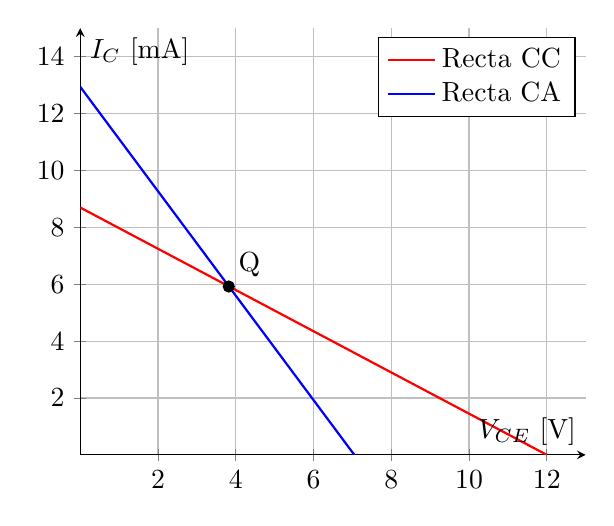
\begin{tikzpicture}
      \begin{axis}[
          axis lines=middle,
          xlabel={$V_{CE}$ [V]},
          ylabel={$I_C$ [mA]},
          xmin=0, xmax=13,
          ymin=0, ymax=15,
          grid=both,
          width=8cm,
          height=7cm,
          xtick={0,2,...,12},
          ytick={0,2,...,14},
      ]
        % Recta de CC: pasa por (0,8.695) y (12,0)
        \addplot[red, thick] coordinates {(0,8.695) (12,0)};
        \addlegendentry{Recta CC}
        % Recta de CA: pasa por (0,12.94) y (7.05,0)
        \addplot[blue, thick] coordinates {(0,12.94) (7.05,0)};
        \addlegendentry{Recta CA}
        % Punto Q
        \addplot[only marks, mark=*] coordinates {(3.82,5.92)};
        \node[above right] at (axis cs:3.82,5.92) {Q};
      \end{axis}
    \end{tikzpicture}
  \end{minipage}
\end{figure}

\section{Simulación}

Una vez hechos los cálculos de diseño y determinados los valores de las resistencias de polarización para el transistor,
considerando el criterio de MES, se procede a realizar una simulación del circuito amplificador. El objetivo de esto es
verificar que los resultados de diseño sean coherentes con el comportamiento real esperado del transistor.

El programa utilizado para la simulación es LTSpice, y el modelo del transistor fue obtenido de la página de un
fabricante, de modo que podemos asegurar que se trata de un modelo válido y funcional. La utilización de un simulador
presenta la ventaja de poder anticipar el desempeño del circuito sin necesidad de un montaje físico, incluyendo
efectos que en los cálculos manuales suelen despreciarse. Por este motivo, los valores obtenidos en simulación pueden
diferir levemente de los calculados en papel, aunque en conjunto ambos métodos permiten predecir de manera confiable el
comportamiento del amplificador antes de su implementación práctica.

En la figura \ref{fig:pto_q_ideal} se muestra la simulación implementada en el programa
mencionado.

\begin{figure}[!ht]
    \centering
    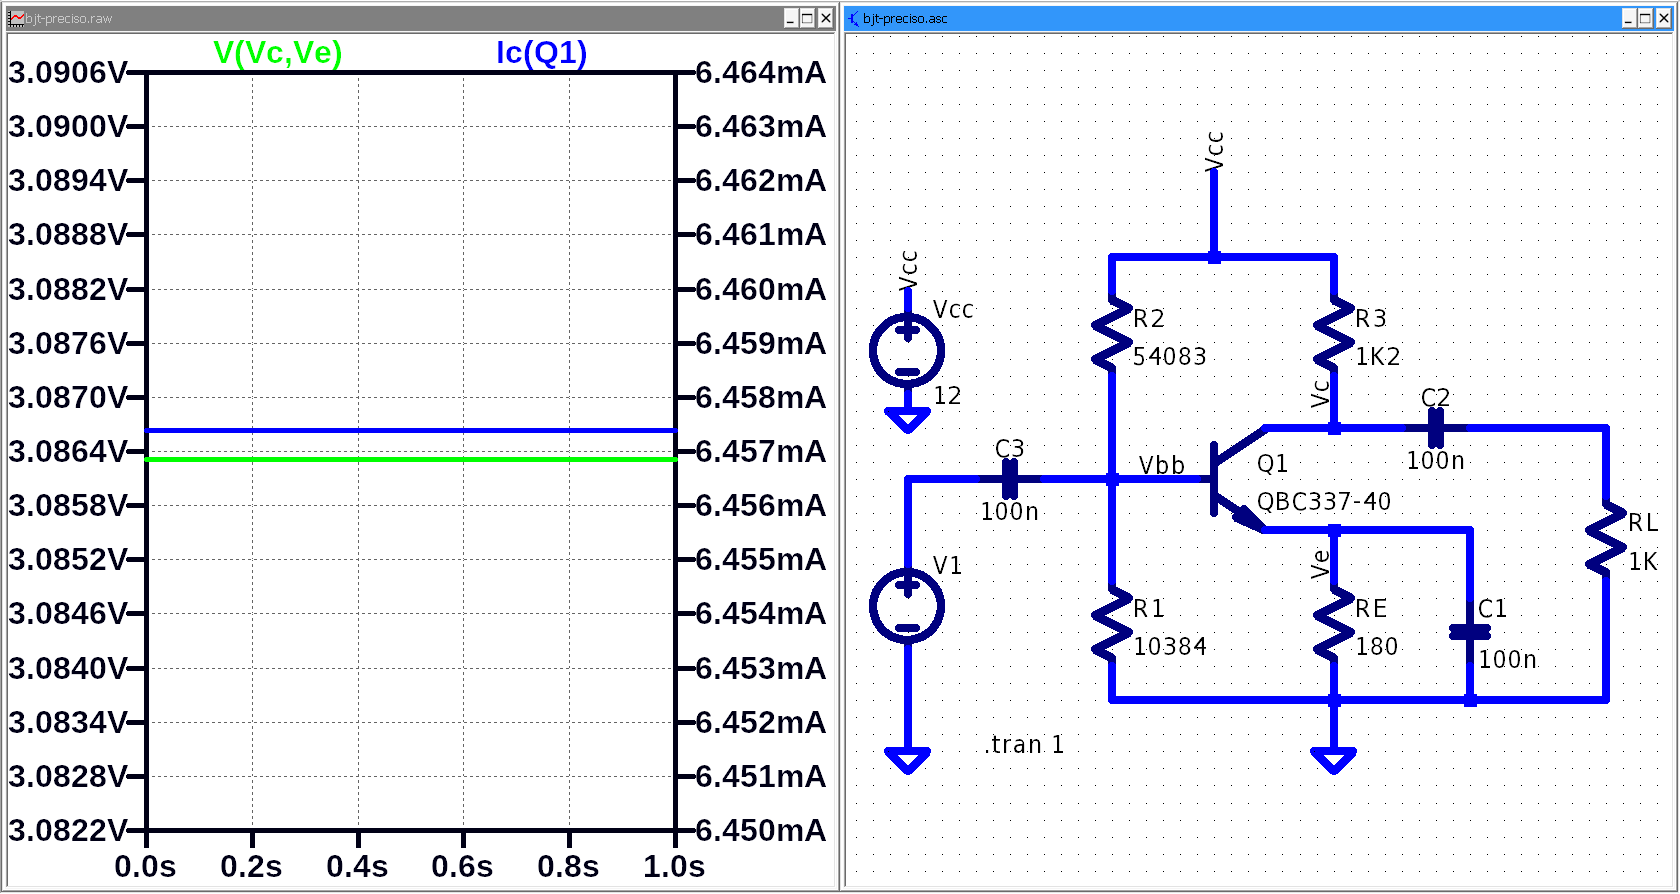
\includegraphics[width=0.5\linewidth]{pto_q_ideal.png}
    \caption{simulación del punto Q con las resistencias obtenidas analíticamente.}
    \label{fig:placeholder}
\end{figure}

Se puede observar que efectivamente hay un poco de discrepancia entre los valores de
$I_{CQ_{MES}}$ y $V_{CEQ_{MES}}$ obtenidos analíticamente y los obtenidos en la simulación.
Sin embargo, los valores de simulación están dentro de un rango de tolerancia de $\pm10\%$
como se puede observar:

Análiticamente se obutuvo $I_{CQ_{MES}} = 6.26mA$, mientras que en la simulación se obtuvo un valor de $I_C = 6.457mA$.
Como se admite una tolerancia de $\pm 10\%$:

\begin{align*}
I_{C,\text{max}} &= 6.26mA + 0.10 \cdot 6.26mA = 6.85mA \\
I_{C,\text{min}} &= 6.26mA - 0.10 \cdot 6.26mA = 5.61mA
\end{align*}

Por lo tanto, el rango de validez es:
\[
5.61mA \leq I_C \leq 6.85mA
\]

Dado que en la simulación $I_C = 6.457mA$, se cumple que:
\[
5.61mA \leq 6.457m \leq 6.85mA
\]

lo cual demuestra que los valores obtenidos mediante los cálculos analíticos y los 
obtenidos mediante simulación son correctos.

Con esto en claro, se puede continuar con la normalización de las magnitudes
de las resistencias $R_1$ y $R_2$. Es decir, se procede a aproximar los valores obtenidos 
mediante cálculos a valores comerciales.
